\documentclass{aa}
% \documentclass[referee]{aa}
\usepackage[varg]{txfonts}
\usepackage[separate-uncertainty=true,
            multi-part-units=single]{siunitx}
\usepackage[version=3]{mhchem}
\usepackage{amsmath}
\usepackage{lscape}
\usepackage{graphicx}
\DeclareMathOperator{\sign}{sign}
\newcommand{\pluseq}{\mathrel{+}=}
\newcommand{\minuseq}{\mathrel{-}=}

\sisetup{range-units = single}
\sisetup{range-phrase = -}

\def\eps{\varepsilon}
\def\aap{A\&A}
\def\eprint{e-prints}
\def\apj{ApJ}
\def\apjs{ApJS}
\def\apjl{ApJL}
\def\mnras{MNRAS}
\def\aj{AJ}
\def\nat{Nature}
\def\aaps{A\&A Supp.}
\def\prd{Phys. Rev. D}
\def\prl{Phys. Rev. Lett.}
\def\araa{ARA\&A}

\begin{document}


\title{SWEET-Cat update and FASMA}
\subtitle{A new minimization procedure for high quality spectra\thanks{Data is
from the following program IDs: 092.C-0695, 093.C-0219,2014B/020, 094.C-0367,
095.C-0324, and 096.C-0092.}}


\author{ D.~T.~Andreasen\inst{1,2}
    \and S.~G.~Sousa\inst{1}
    \and M.~Tsantaki\inst{3}
    \and G.~Teixeira\inst{1}
    \and A.~Mortier\inst{4}
    \and N.~C.~Santos\inst{1,2}
    \and L.~Su\'arez-Andr\'es\inst{5,6}
    \and E.~Delgado-Mena\inst{1}
}


\institute{
Instituto de Astrof\'isica e Ci\^encias do Espa\c{c}o, Universidade do Porto, CAUP, Rua das Estrelas, 4150-762 Porto, Portugal
\email{daniel.andreasen@astro.up.pt}
\and
Departamento de F\'isica e Astronomia, Faculdade de Ci\^encias, Universidade do Porto, Rua Campo Alegre, 4169-007 Porto, Portugal
\and
Instituto de Radioastronom\'ia y Astrof\'isica, IRyA, UNAM, Campus Morelia, A.P. 3-72, 58089 Michoac\'an, Mexico
\and
SUPA, School of Physics and Astronomy, University of St Andrews, St Andrews KY16 9SS, UK
\and
Depto. Astrof\'isica, Universidad de La Laguna (ULL), E-38206 La Laguna, Tenerife, Spain
\and
Instituto de Astrof\'isica de Canarias, E-38205 La Laguna, Tenerife, Spain
}





\date{Received ...; accepted ...}

\abstract
% Context
{}
% Aims
{}
% Methods
{}
% Results
{}
% Conclusions
{}



\keywords{data reduction: high resolution spectra --
          stars individual: Arcturus --
          stars individual: HD010853}
\maketitle



\section{Introduction}
\label{sec:introduction}
The study of extrasolar planetary systems is an established field of research.
To date, nearly 3500 extrasolar planets have been discovered around almost 2500
solar-type stars\footnote{For an updated table we refer to
\url{http://www.exoplanet.eu}}. Most of these have been found thanks to the
incredible precision achieved in photometric transit and radial velocity
methods. Not only do we have intriguing new types of planetary systems that
challenge current theories but also the increasing number of exoplanets allows
us to do statistical studies of the newfound worlds by analyzing their internal
structure, atmospheric composition, and planetary composition.

Precise and accurate planetary parameters (mass, radius, and mean density) are
needed to distinguish between solid rocky, water rich, gaseous, or otherwise
composed planets. A key aspect to this progress is the characterization of the
planet host stars. For instance, precise and accurate stellar radii are critical
if we want to measure precise and accurate values of the radius of a transiting
planet \citep[see e.g.][]{Torres2012,Mortier2013}. The determination of the
stellar radius is in turn dependent on the quality of the derived stellar
atmospheric parameters such as the effective temperature.

We continue the work of \citet{Santos13} by deriving atmospheric parameters,
namely the effective temperature ($T_\mathrm{eff}$), surface gravity ($\log g$),
metallicity ([Fe/H], where iron often is used as a proxy for the total
metallicity), and the micro turbulence ($\xi_\mathrm{micro}$) in a homogeneous
way for a sample of planet host stars. This, in turn, allows us to study new
correlations between planets and their hosts in a homogeneous way,  or gain
higher statistical certainty on the already discovered correlations.

The analysis of high quality spectra, i.e. spectra with high spectral resolution
and an high  signal to noise ratio (SNR), serves an important role in the
derivation of stellar atmospheric parameters. Nevertheless, spectral analysis is
a time consuming method. There has been an increase of the amount of  optical
high-resolution spectrographs available and, additionally, a number of near-IR
spectrographs are either planned or are already available making the task of
analyzing the increasing amount of spectra even more crucial.

In the era of large data sets, computation time has to be decreased as much as
possible without compromising the quality of the results. In the light of this
we have developed a tool to derive atmospheric parameters in a fast and robust
way using standard spectroscopic methods. We made this tool available as a web
interface at \url{link to FASMA}. This works well for optical spectra which we
demonstrate in Section~\ref{sub:Testing_FASMA} using the line list from
\citet{Sousa2011}. This tool also ships with a line list for near-IR spectra
using the line list presented recently in \citet{Andreasen2016}. The tool is
provided to the community as an easy to use web tool to avoid any problems with
installations. The tool is described in detail in Section~\ref{sec:FASMA}.



\section{Data}
\label{sec:data}
In this paper we derived parameters for a sample 66 stars,
43 were observed by our team using the UVES \citep{UVES}, FEROS
\citep{FEROS}, and FIES \citep{FIES} spectrographs. The rest (23) spectra were
found in various archives. Additionally, we use spectra from HARPS \citep{HARPS}
and ESPaDOnS \citep{ESPADONS}. Some characteristics of the spectrographs are
presented in Table~\ref{tab:instruments} with the mean SNR for the spectra used.
The SNR for each star can be seen in Table~\ref{tab:results} along with the
atmospheric parameters of the stars.

We obtain the spectra with the highest possible resolution for a given
spectrograph, and in cases with multiple observations, we include all unless a
spectrum is close to the saturation limit for a given spectrograph. For multiple
spectra, we combine them after first correcting the radial velocity (RV) and
using a sigma clipper to remove cosmic rays. The individual spectra are then
combined to a single spectrum for a given star to increase the SNR. This single
spectrum is used in the analysis below. For most of the spectra in the archive
included here, several spectra were combined as described above, while for the
observations dedicated to this work, the spectrum would be a single spectrum.
This is mostly due to the difference in science cases behind the observations.
E.g. the HARPS spectra were used for RV monitoring or follow up of the
exoplanet(s), while the UVES spectra were used for characterisation of stellar
parameters.

\begin{table}[htb!]
    \caption{Spectrographs used for this paper with their spectral resolution,
             wavelength coverage, and typical (mean) SNR from the spectra used.}
    \label{tab:instruments}
    \centering
    \begin{tabular}{llll}
      \hline\hline
      Spectrograph & Resolution & Spectral coverage           &   Mean SNR  \\
      \hline
      UVES         &    110 000 & $\SIrange{480}{680}{nm}$    &   212       \\
      FEROS        &     48 000 & $\SIrange{350}{920}{nm}$    &   208       \\
      HARPS        &    115 000 & $\SIrange{378}{691}{nm}$    &   642       \\
      FIES         &     67 000 & $\SIrange{370}{730}{nm}$    &   763       \\
      ESPaDOnS     &     81 000 & $\SIrange{370}{1050}{nm}$   &   775       \\
      \hline
    \end{tabular}
\end{table}




\section{FASMA}
\label{sec:FASMA}
FASMA (acronym for Fast Analysis of Spectra Made Automatically) is a web
tool\footnote{\url{super-cool-address-with-FASMA}} for analyzing spectra. FASMA
is written in Python and works as a wrapper around MOOG
\citep[][version 2014]{Sneden1973}, and ARES \citep{Sousa2015a} for an all-in-one
tool. MOOG is a radiative transfer code under the assumption of local
thermodynamic equilibrium (LTE). ARES is a tool to automatically measure
equivalent widths (EW) from a spectrum given a line list. FASMA has three
different modes: i) Measure EWs using ARES, ii) derive stellar parameters from a
set of measured \ion{Fe}{I} and \ion{Fe}{II} line EWs, and iii) abundances
derivation for 15 elements, all described below. The model atmospheres are
formatted in a grid of Kurucz Atlas 9 plane-parallel, 1D static model
atmospheres \citet{Kurucz1993}. FASMA can also manage the new grid of Atlas
models calculated by \citet{Meszaros2012} for the APOGEE survey and the MARCS
models \citep{Gustafson2008}. The interpolation from the grid is calculated from
a geometric mean for effective temperature, surface gravity and metallicity.



\subsection{EW measurements}
\label{sub:EW_measurements}
The EWs are strongly correlated with the atmospheric parameters. Measurements of
the EW can be done manually using a tool like splot in IRAF, but often when
dealing with a large sample of stars this is not a suitable way to deal with the
task. Therefore tools like ARES exist which can measure the EWs of spectral
lines automatically. To use this mode of FASMA, it just needs a spectrum (format
should be 1D fits for ARES to read it) and a line list. For the latter, FASMA is
shipped with some line lists ready to use, in the format suitable for FASMA. The
output will be a line list in the format required for MOOG. The output can be
used for either the EW method or the abundance method, both described below.

The line lists shipped with FASMA are presented in Table~\ref{tab:linelists}.
These line lists are all calibrated for the Sun, i.e. the oscillator strengths
for each absorption line are changed so the line with the measured EW from a
solar spectrum return solar abundance for the given element.

\begin{table}[htb!]
    \caption{The line lists provided with FASMA. The first two line lists
             are for parameter determination while the last line list is
             used to derive abundances for 15 different elements.}
    \label{tab:linelists}
    \centering
    \begin{tabular}{lrrl}
      \hline\hline
      Line list             & \ion{Fe}{I}/\ion{Fe}{II} & Elements   & Usage      \\
      \hline
      \citet{Sousa2008a}    &  263/36                  &  1         & Parameters \\
      \citet{Tsantaki2013}  &  120/17                  &  1         & Parameters \\
      \citet{Andreasen2016} &                          &  1         & Parameters \\
      \citet{Neves2009}     &  -/-                     & 15         & Abundances \\
      \hline
    \end{tabular}
\end{table}



\subsection{EW method}
\label{sub:EW_method}
The standard determination of spectroscopic parameters for solar-type stars
starts by measuring the EW of selected and well-defined absorption lines. Then
we translate these measurements into individual line abundances, assuming a
given atmospheric model. We obtain the correct stellar parameters by imposing
excitation and ionization balance for the iron species.

\begin{itemize}
    \item The effective temperature has a strong influence on the correlation
          of iron abundance with the excitation potential (excitation balance).
          We obtain the $T_\mathrm{eff}$ when \ion{Fe}{I} abundance shows no
          dependence on the excitation potential, i.e., the slope of abundance
          versus excitation potential is zero.
    \item Surface gravity is derived from the ionization balance of \ion{Fe}{I}
          and \ion{Fe}{II} abundances. Therefore, the abundance of neutral iron
          should be equal to the abundance of ionized and consistent with the
          one of the input model atmosphere.
    \item Microturbulence is connected with the saturation of the stronger iron
          lines. However, the abundances for weak and strong lines of a certain
          species (in our case iron) should be the same independent of the value
          of $\xi_\mathrm{micro}$. Iron abundances should show no dependence on
          the reduced equivalent width, i.e. the slope of abundance vs the
          reduced EW is zero.
\end{itemize}


With measured EWs of \ion{Fe}{I} and \ion{Fe}{II} lines we calculate abundances
using a stellar atmosphere model for a given set of atmospheric parameters
($T_\mathrm{eff}$, $\log g$, [Fe/H], and $\xi_\mathrm{micro}$). By removing
correlations between the measured abundances (through the measured EWs) and the
excitation potential (EP) and reduced EW ($\log(EW/\lambda)$) we can constrain
$T_\mathrm{eff}$ and $\xi_\mathrm{micro}$. By obtaining ionization balance
between \ion{Fe}{I} and \ion{Fe}{II} (that is the average abundance of all
\ion{Fe}{I} lines are equal to the average abundance of all \ion{Fe}{II} lines)
we constrain $\log g$. Lastly, we change the input [\ion{Fe}/\ion{H}] to match
that of the average output [\ion{Fe}/\ion{H}]. Hence we have four criteria to
minimize simultaneously:

\begin{enumerate}
    \item The slope between abundance and excitation potential ($a_\mathrm{EP}\le0.001$).
    \item The slope between abundance and reduced EW ($a_\mathrm{RW}\le0.003$).
          We use 0.003 rather than 0.001 since this slope varies more rapidly
          with small changes in atmospheric parameters.
    \item The difference between the average abundances of \ion{Fe}{I} and
          \ion{Fe}{II} ($\Delta\ion{Fe}{}\le0.01$).
    \item Input and output metallicity should be equal.
\end{enumerate}
These criteria we denote as indicators for the physical parameters which we are
trying to minimize for. We denote this method for obtaining stellar parameters
for the EW method.

\begin{figure}[tpb]
    \centering
    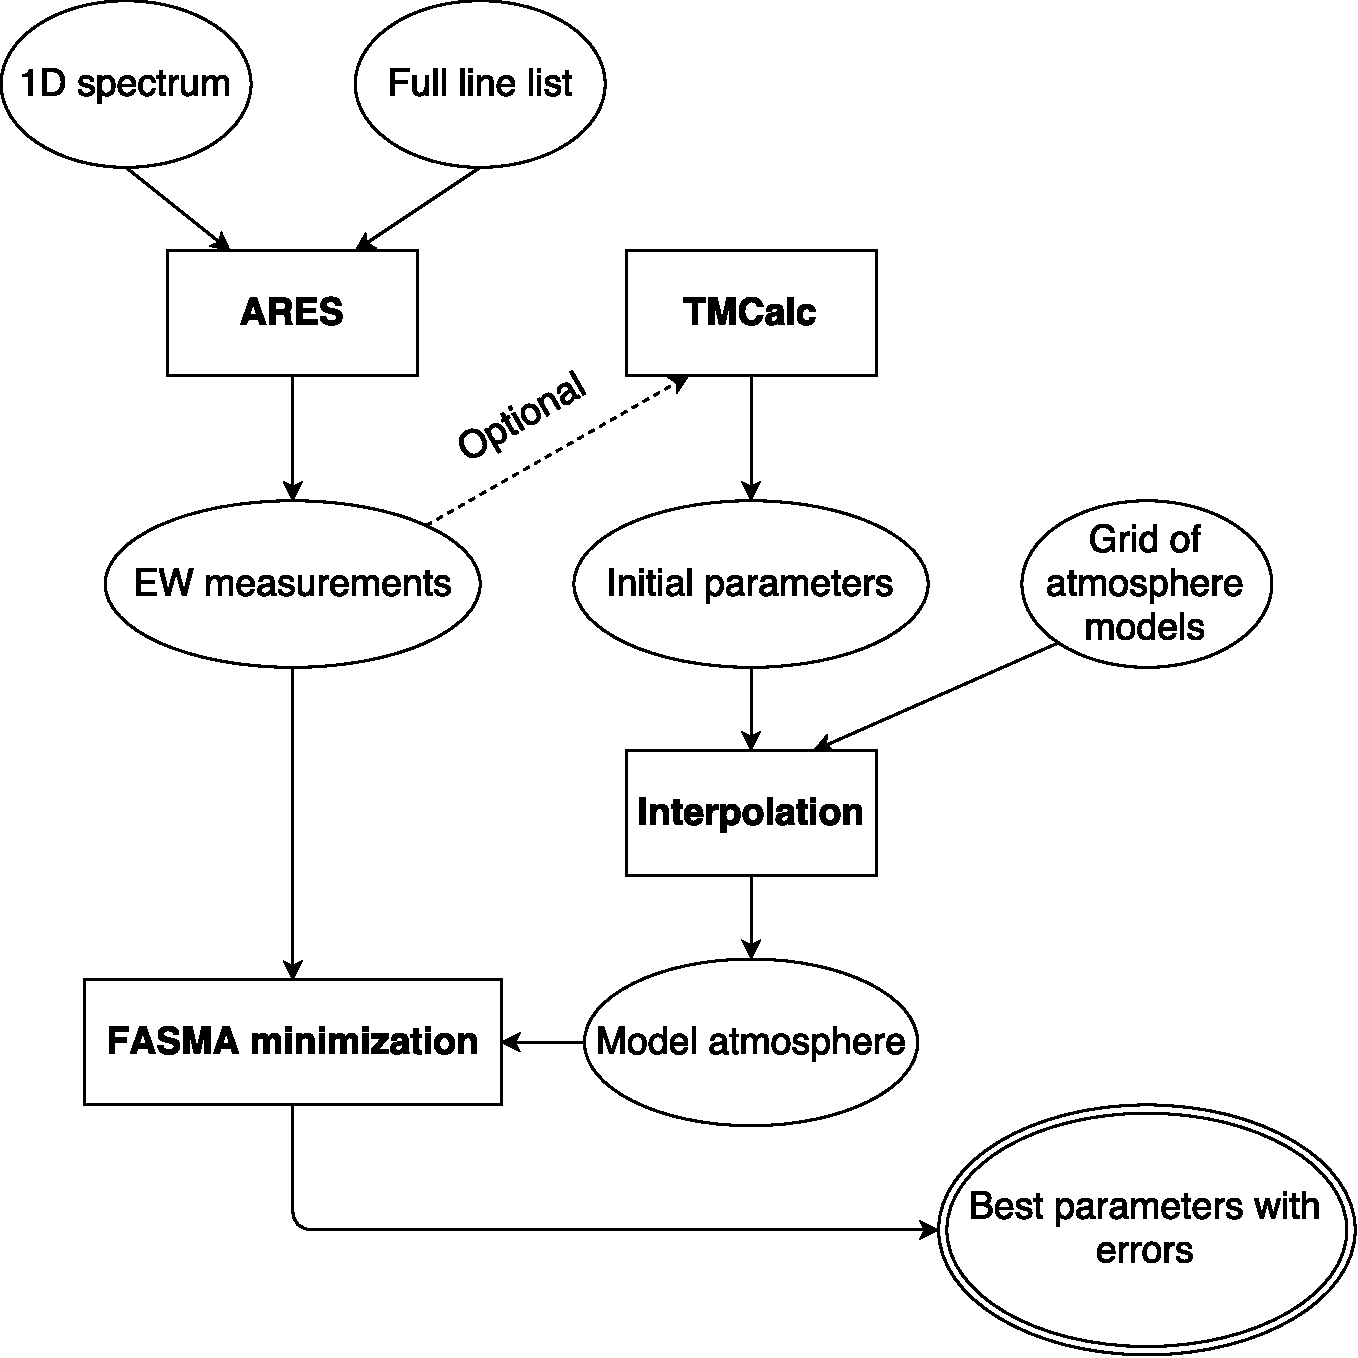
\includegraphics[width=1.0\linewidth,natwidth=700,natheight=650]{figures/FASMA_general.pdf}
    \caption{A general overview over FASMA from spectrum to parameters.}
    \label{fig:FASMA_general}
\end{figure}

There exists many minimization routines available in Python. Most commonly known
are the ones from the SciPy ecosystem\footnote{\url{http://scipy.org}}. There
are some pros and cons with using proprietary minimization routines. Pros are
that it is already written, and usually there is good documentation for
libraries such as SciPy. Cons in this situation is, that most minimization
routines do not work well with vector functions returning another vector:
\begin{align}
    f(\{T_\mathrm{eff}, \log g, [Fe/H], \xi_\mathrm{micro}\}) = \{a_\mathrm{EP}, a_\mathrm{RW}, \Delta\ion{Fe}, \ion{Fe}{I}\}.
\end{align}
A work around is to combine the criteria into one single criteria by e.g. adding
them quadratically and minimize that expression instead. Thus we have a vector
function returning a scalar:
\begin{align}
    f(\{T_\mathrm{eff}, \log g, [Fe/H], \xi_\mathrm{micro}\}) &= \sqrt{a_\mathrm{EP}^2 + a_\mathrm{RW}^2 + \Delta\ion{Fe}{}^2}.
\end{align}
The minimization routines are also not physical in the sense that they are not
optimized for the problem. These two cons were incitement for writing a
minimization routine optimized for the problem at hand. Here is how it works.

\begin{enumerate}
    \item Run MOOG once with a user defined initial parameters (default is
          solar) and calculate $a_\mathrm{EP}$, $a_\mathrm{RW}$, and
          $\Delta$\ion{Fe}.
    \item Change the atmospheric parameters ($T_\mathrm{eff}$, $\log g$,
          [\ion{Fe}/\ion{H}], $\xi_\mathrm{micro}$) according to the size of the
          indicator. A parameter is only changed if it is not fixed.
    \begin{itemize}
        \item $a_\mathrm{EP}$: Indicator for $T_\mathrm{eff}$. If this value
              is positive, then increase $T_\mathrm{eff}$.
        \item $a_\mathrm{RW}$: Same as above but for $\xi_\mathrm{micro}$.
        \item $\Delta$\ion{Fe}{}: Positive $\Delta$\ion{Fe}{} means $\log g$
              should be decreased and vice versa.
        \item For [\ion{Fe}/\ion{H}] it is changed to the output [\ion{Fe}/\ion{H}]
              in each iteration.
    \end{itemize}
    \item If the new parameters have already been used in a previous iteration,
          then change them slightly. This is done by drawing a random number from
          a Gaussian distribution with a mean at the current value and a sigma
          equal to the absolute value of the indicator.
    \item Calculate a new atmospheric model by interpolating a grid so we have
          the requested parameters and run MOOG once again.
    \item For each iteration save the parameters used and the quadratic sum of
          the indicators. If we do not reach convergence, then return the best
          found parameters.
\end{enumerate}
This whole process is schematically shown in Figure~\ref{fig:FASMA_general} and
the minimization routine itself in Figure~\ref{fig:FASMA_minimization}. The
stepping follows these simple equations:
\begin{align}
    T_\mathrm{eff}     &\pluseq \SI{2000}{K} a_\mathrm{EP}   \\
    \xi_\mathrm{micro} &\pluseq \SI{1.5}{km/s} a_\mathrm{RW} \\
    \log g             &\minuseq \Delta\ion{Fe}.
\end{align}
The metallicity is corrected at each step so the input metallicity matches that
of the output metallicity of the previous iteration. The functional form for
changing the parameters were found by changing one parameter, e.g.
$T_\mathrm{eff}$, while keeping the other parameters fixed at their convergence
values. A linear fit was applied to $T_\mathrm{eff} - T_\mathrm{eff,0}$ vs.
$a_\mathrm{EP}$ in order to get the slope. Since we ignore all interdependencies
between the parameters in doing so, we lower the slopes above a little and
arrive to these very simple equations.

The error estimates are based on the same method presented in
\citet{Gonzalez2000}, which is also described in details in
\citet{Santos2003,Andreasen2016}.

\begin{figure}[tpb]
    \centering
    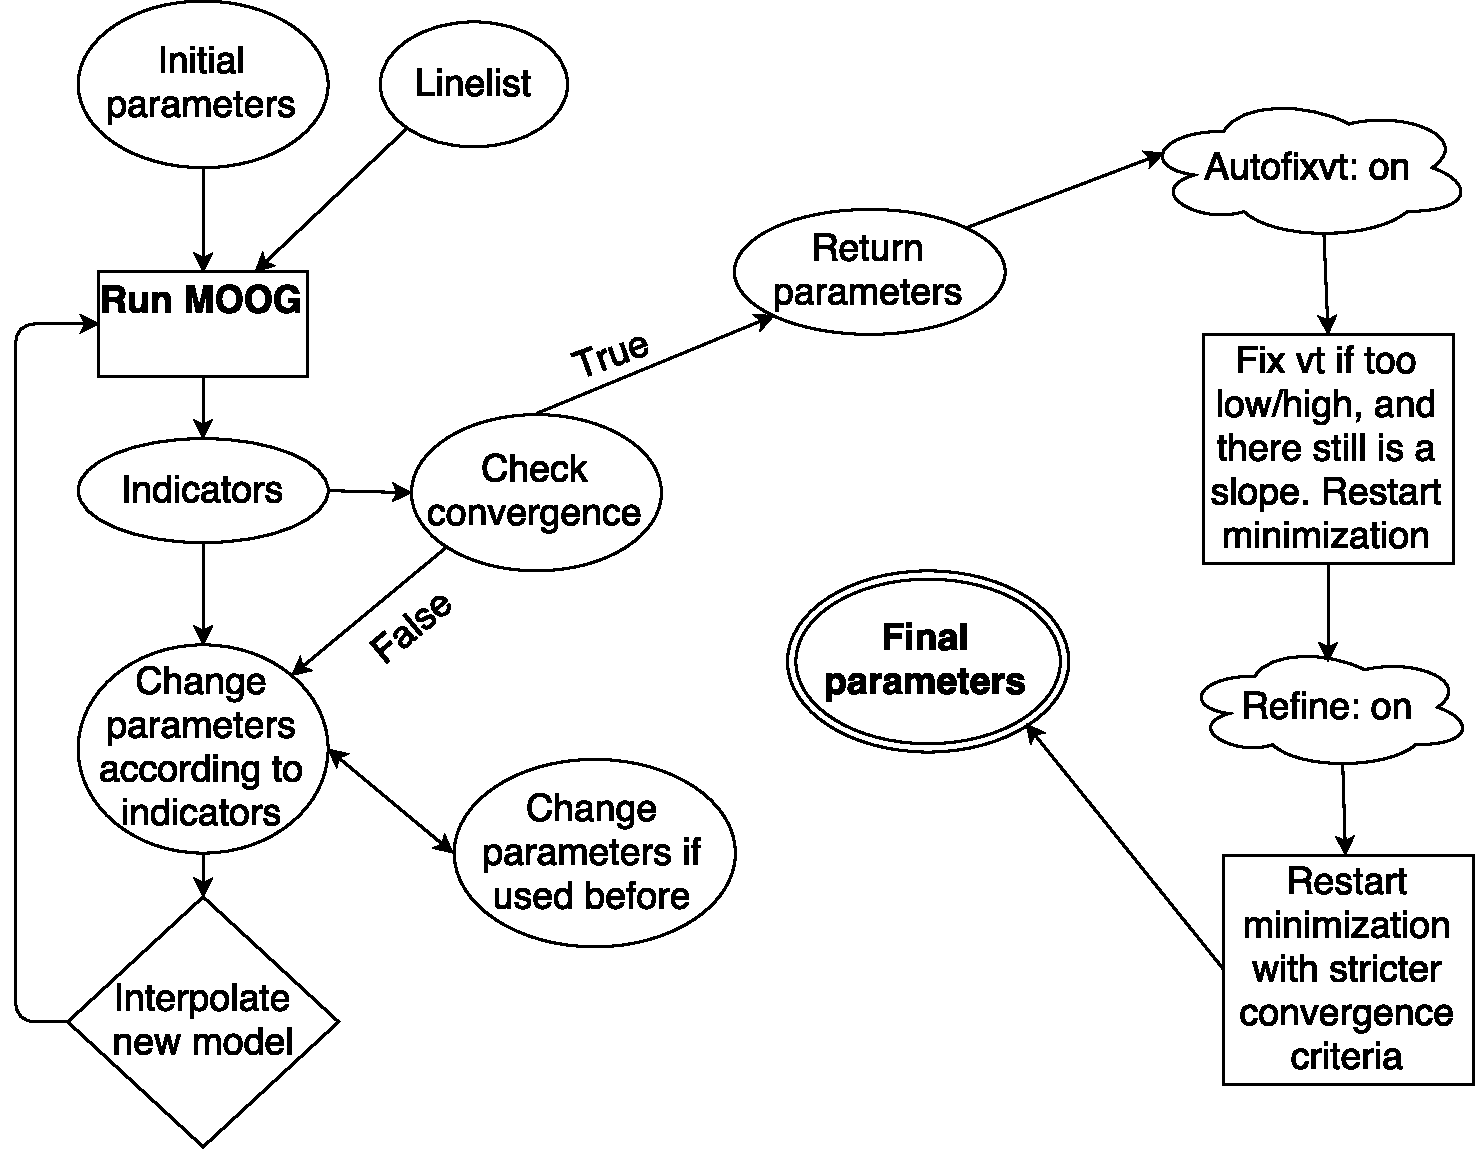
\includegraphics[width=1.0\linewidth,natwidth=700,natheight=650]{figures/FASMA_minimization.pdf}
    \caption{A schematic overview over the minimization for FASMA with the
    EW method.}
    \label{fig:FASMA_minimization}
\end{figure}

By using the indicators like this, we can relative fast reach convergence.
Typical calculation time for an FGK dwarf with a high quality spectrum is around
$\SI{2}{min}$.

\subsubsection{Options}
\label{subs:EWoptions}
It is possible to run the EW method with a set of different options which
will be described here.

\begin{itemize}
    \item \emph{fixteff}: Fix $T_\mathrm{eff}$ and derive the other parameters.
          Same is available for $\log g$ (\emph{fixlogg}), [\ion{Fe}/\ion{H}]
          (\emph{fixfeh}), and $\xi_\mathrm{micro}$ (\emph{fixvt}). One or more parameters
          can be fixed. When one or more parameters are fixed, the corresponding
          indicator will be ignored for each iteration, thus the parameter itself
          will not be changed.
    \item \emph{outlier}: Remove outliers after the first run with the minimization
          routine and restarting the minimization from the previous best
          parameters. The options are to remove all outliers above $3\sigma$
          once or iteratively, or remove one outlier above $3\sigma$ once or
          iteratively.
    \item \emph{autofixvt}: If the minimization routine does not converge and
          $\xi_\mathrm{micro}$ is close to 0 or 10 with a significant
          $a_\mathrm{RW}$ (numerically bigger than 0.05), then fix
          $\xi_\mathrm{micro}$. This option was added since we saw this behaviour
          in some cases. The solution was typically to restart the minimization
          manually with $\xi_\mathrm{micro}$ fixed.
    \item \emph{refine}: After the minimization is done, run it again from the best
          found parameters but with more strict criteria. If this option is set,
          it will always be the last step (after removal of outliers). The
          convergence criteria can be changed by the user, but we recommend
          using the defaults provided above.
    \item \emph{tmcalc}: Use TMCalc \citep{Sousa2012} to fast estimate the
          $T_\mathrm{eff}$ and $[\ion{Fe}/\ion{H}]$ using the raw output from
          ARES. We then assume solar surface gravity ($\SI{4.44}{dex}$) and
          estimate $\xi_\mathrm{micro}$ based on an empirical relation (see below).
\end{itemize}
If $\xi_\mathrm{micro}$ is fixed it is changed at each iteration according to an
empirical relation. For dwarfs it follows the one presented in
\citet{Tsantaki2013} and for giants it follows the one presented in
\citet{Adibekyan2015}.

We use the line list presented in \citet{Sousa2008a}. However, this line list
does not work well for cool stars. This was fixed in \citet{Tsantaki2013} by
removing some lines from \citet{Sousa2008a}. For stars cooler than \SI{5200}{K}
we automatically rederive the atmospheric parameters after removing lines so the
line list resemble that of \citet{Tsantaki2013}.

All restarts of the minimization routine is done with initial condition at the
last found best parameters.


\subsection{Abundance method}
\label{sub:Abundance_method}

With the line list from \citet{Neves2009} with 15 different elements it is
possible to measure abundances for these elements by combining the ARES mode to
measure the EWs and the EW method mode to obtain the atmospheric parameters. The
abundances are saved to a table.


\subsection{Testing FASMA}
\label{sub:Testing_FASMA}
To test the EW method implemented in FASMA we derive parameters from the 582
sample by \citet{Sousa2011}. This sample has a wider range of SNR than the 451
sample from \citet{Tsantaki2013}, therefore making it better for a comparison.
We use ARES2 to measure the EWs. ARES can give an estimate on the signal to
noise ratio (SNR) by analyzing the continuum in given intervals. For solar type
stars the following intervals are working well: \SIrange{5764}{5766}{\angstrom},
\SIrange{6047}{6053}{\angstrom}, and \SIrange{6068}{6076}{\angstrom}. From the
estimated SNR, ARES can give an estimate on the very important \emph{rejt}
parameters \citep[see][for more information]{Sousa2015a}. After measuring the
EWs with ARES, we use the FASMA minimization described in
Section~\ref{sub:EW_method} to determine the stellar atmospheric parameters. The
results are presented in Figure~\ref{fig:FASMATest} which shows
$T_\mathrm{eff}$, $\log g$, [\ion{Fe}/\ion{H}], and $\xi_\mathrm{micro}$ for
FASMA against those of \citet{Sousa2011}.

\begin{figure*}[tpb]
    \centering
    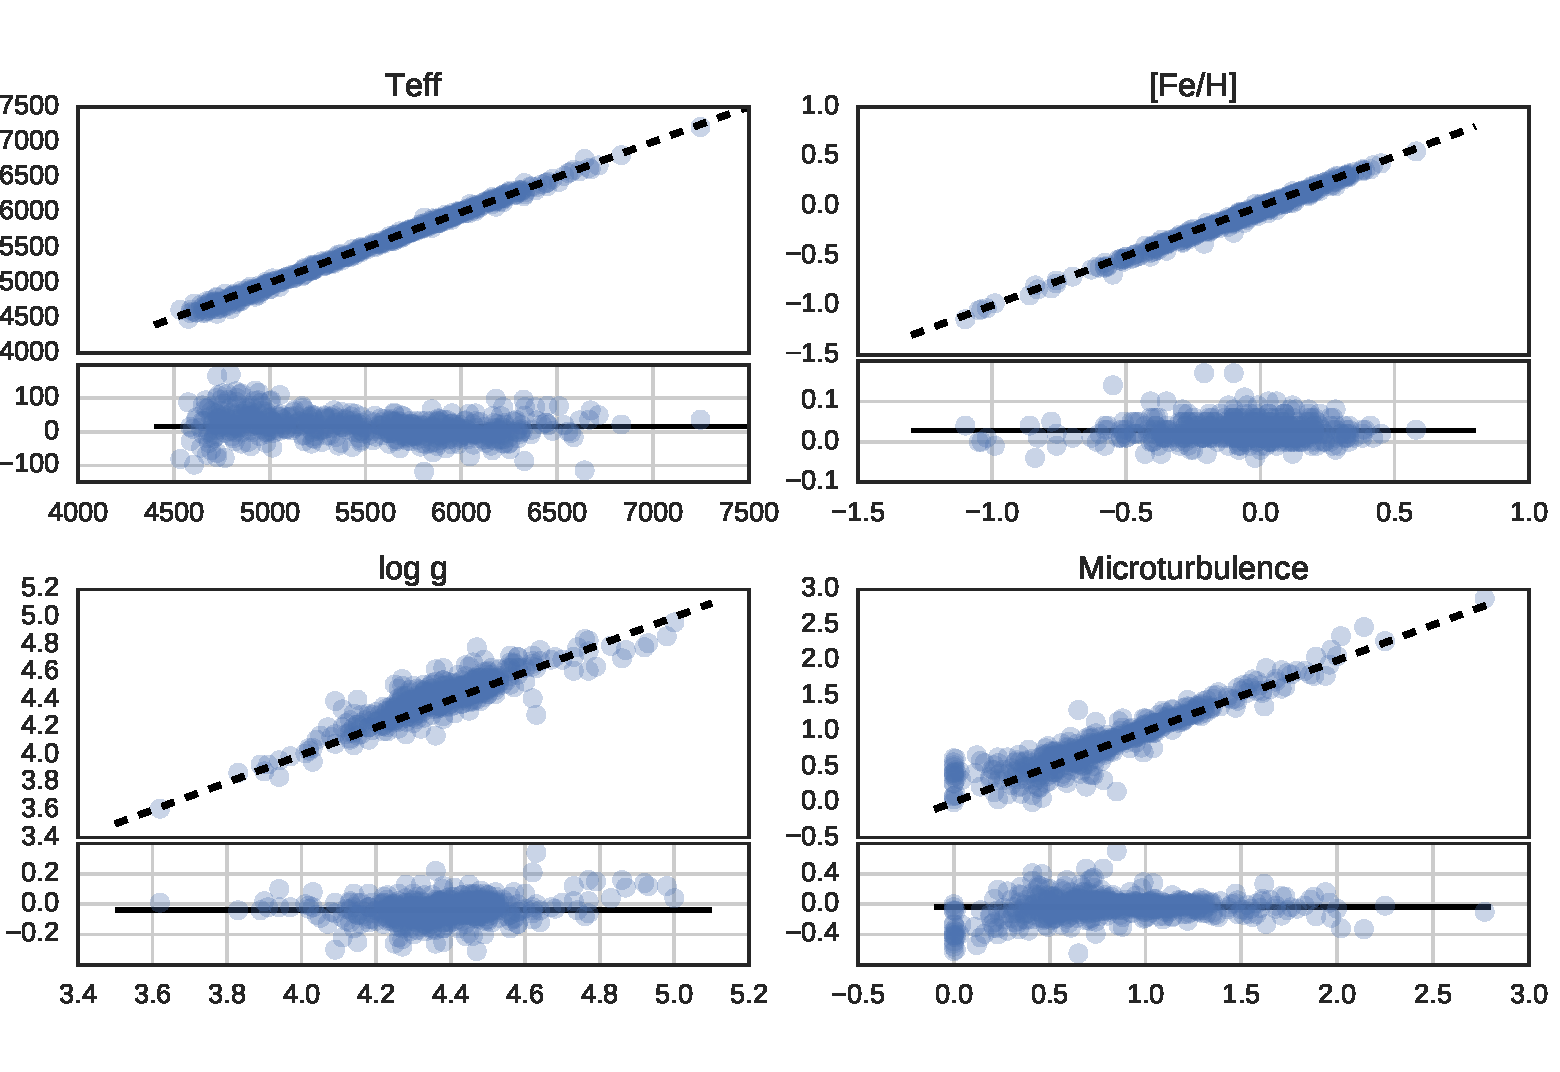
\includegraphics[width=1.0\linewidth,natwidth=750,natheight=500]{figures/FASMATest.pdf}
    \caption{Stellar atmospheric parameters derived by FASMA compared
    to the sample by \citet{Sousa2011}. The x-axis in all plots show the results
    from FASMA while the y-axis is the parameters derived by \citet{Sousa2011}.}
    \label{fig:FASMATest}
\end{figure*}

The sample contains stars with $T_\mathrm{eff}$ too cold for the line list used.
As described in Section~\ref{sub:EW_method} we should then convert the line list
by \citet{Sousa2008a} to the line list presented in \citet{Tsantaki2013}.
However, since this line list was not available when \citet{Sousa2011} derived
parameters, we do not make this change in order to make a fair comparison for
FASMA.

The mean of the difference between parameters from \citet{Sousa2011} and those
by FASMA are presented in Table~\ref{tab:FASMATest}.

\begin{table}[htb!]
    \caption{The difference in derived parameters by \citet{Sousa2011}
    and FASMA. Second column is the mean difference with EWs measured by
    ARES in FASMA, while the third column is the mean difference using
    20 randomly stars with the exact same line list.}
    \label{tab:FASMATest}
    \centering
    \begin{tabular}{lrr}
      \hline\hline
      Parameter             &  Mean difference         & Same line list        \\
      \hline
      $T_\mathrm{eff}$      &  $\SI{16(36)}{K}$        & $\SI{21(11)}{K}$      \\
      $\log g$              &  $\num{-0.04(7)}$        & $\num{-0.007(9)}$     \\
      $[\ion{Fe}/\ion{H}]$  &  $\num{0.03(2)}$         & $\num{0.004(9)}$      \\
      $\xi_\mathrm{micro}$  &  $\SI{-0.04(14)}{km/s}$  & $\SI{0.04(2)}{km/s}$  \\
      \hline
    \end{tabular}
\end{table}

The comparison is very consistent as expected and the small offsets are within
the errors except for metallicity. This can be due to different versions of
MOOG, measured line lists, interpolation of atmosphere grid, and minimization
routine. Most likely the difference will be due to different used \emph{rejt}
parameters in ARES, which can alter the EWs systematically and hence the
metallicity. We therefore randomly selected 20 stars with different
$T_\mathrm{eff}$ and used the line lists directly from \citet{Sousa2011} to
derive parameters. The results are presented in the last column of
Table~\ref{tab:FASMATest}. We note that the $\log gf$ values from the original
line lists by \citet{Sousa2011}, which used the MOOG 2002 version, were not
changed for the 2014 version of MOOG. This might lead to some errors as well.
However, the offsets are very small and compatible with the errors on parameters
normally obtained from high quality spectra.


\subsection{Web interface}
\label{sub:Web interface}
NOTE: More will be written once we have a web page.

We provide a web interface for FASMA. In the web interface it is possible to use
some of the line list provided with FASMA to measure EWs of a spectrum (has to
be provided by the user). This can be used for all the available FASMA methods
described above.

The web interface can be found at the following link
\url{super-cool-address-with-FASMA}.



\section{New homogeneous spectroscopic parameters for 66 planet hosts}
\label{sec:results}
Here we present the sample of 66 stars. We were unable to derive parameters for
HD77065. This is a spectroscopic binary according to \cite{Pourbaix2004}, and
the spectrum is contaminated with the companion star. This make EW measurement
very difficult, hence we exclude it from the sample of collected spectra.

Moreover we were not able to successfully derive parameters with this method for
Aldebaran, a well known red giant star. Even though the quality of the spectra
for a bright star like Aldebaran are available, the spectral type is intrinsic
difficult due to the low $T_\mathrm{eff}$ which can give arise to molecular
absorption in the optical. We also expect to see non-LTE effects for this kind
of spectral type. That we are not able to derive parameters for Aldebaran is not
a big concern, since it is well studied with other techniques, and we can trust
the parameters already listed in SWEET-Cat.

Last, we also removed .... from our sample since these stars did not convergence
during the minimization procedure. The $T_\mathrm{eff}$ for these stars are too
high for the EW method to work.

The remaining 66 stars are presented in Table~\ref{tab:results}. Note that we
apply a correction to the spectroscopic $\log g$ based on asteroseismology as
found in \citet{Mortier2014}. We only use this corrections for FGK dwarf stars,
i.e. between $\SI{4800}{K}\leq T_\mathrm{eff} \leq \SI{6500}{K}$ and
$\log g\geq4.2$. For stars with a $\log g$ lower than this limit we do not apply
the corrections, and if the $\log g$ change to below this limit after the
correction, we go back to use the spectroscopic $\log g$ again.

We present a Hertzprung-Russel diagram (HRD) of our sample in
Figure~\ref{fig:HRD}. Figure~\ref{fig:HRD} is made with a tool for post
processing the results saved to a table by FASMA.

\begin{figure}[tpb]
    \centering
    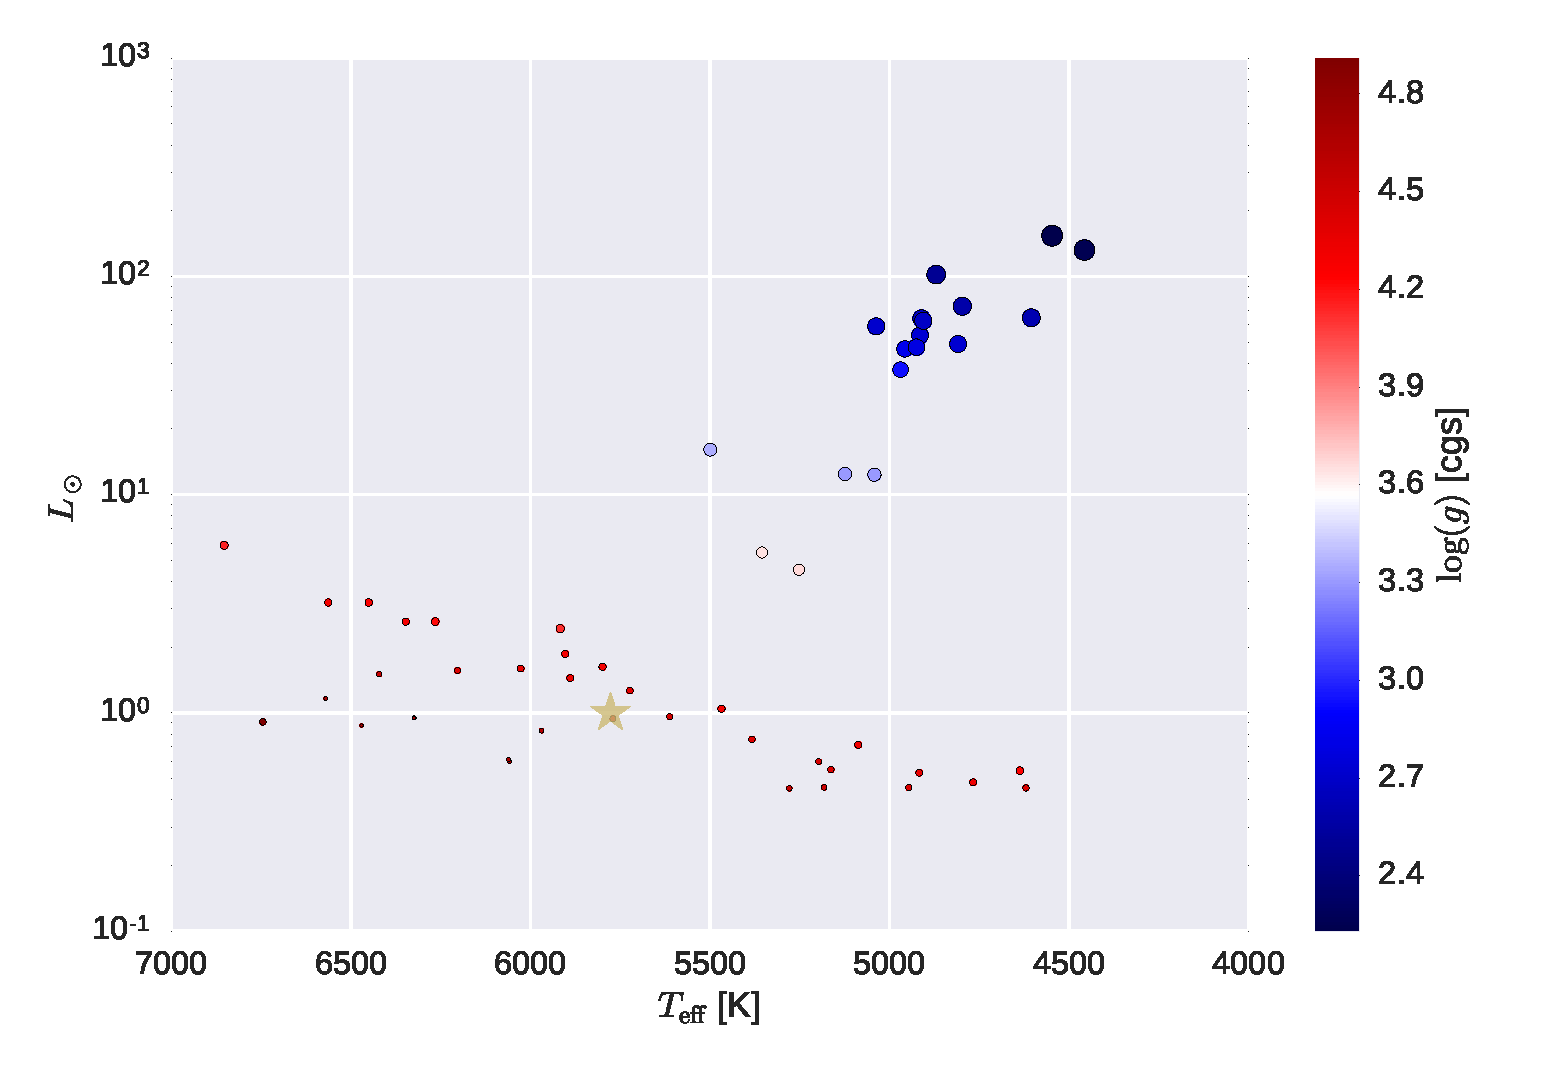
\includegraphics[width=1.0\linewidth,natwidth=440,natheight=290]{figures/HR.pdf}
    \caption{Hertzprung-Russel diagram of our sample with the Sun as a green
    star. The size of the points represents the $\log g$, with bigger points
    being smaller $\log g$ (giants), and vice versa. The colour code show the
    same as the size. Red points are the dwarfs, while yellow points are the
    giants.}
    \label{fig:HRD}
\end{figure}

We present the new atmospheric parameters in Figure~\ref{fig:update} against the
same parameters before the update. With 2461 stars discovered with planets, 21\%
of these stars have been analyzed in the homogeneous way as described in this
work. We note that the limiting factor at the moment for increasing the sample
of stars analyzed in the homogeneous way is the magnitude of that planet hosts.
There have been found many planet hosts with space mission as \emph{Kepler} and
\emph{CoRoT} using the transiting method. Most of these stars are faint and thus
making them time expensive for the spectroscopic analysis required here. For
stars brighter than magnitude 12 the completeness, i.e. the stars analyzed in a
homogeneous way compared to the ones we did not analyze yet, is up to 77\% now
while it is at 85\% for exoplanet hosts brighter than magnitude 10.

\begin{figure*}[tpb]
    \centering
    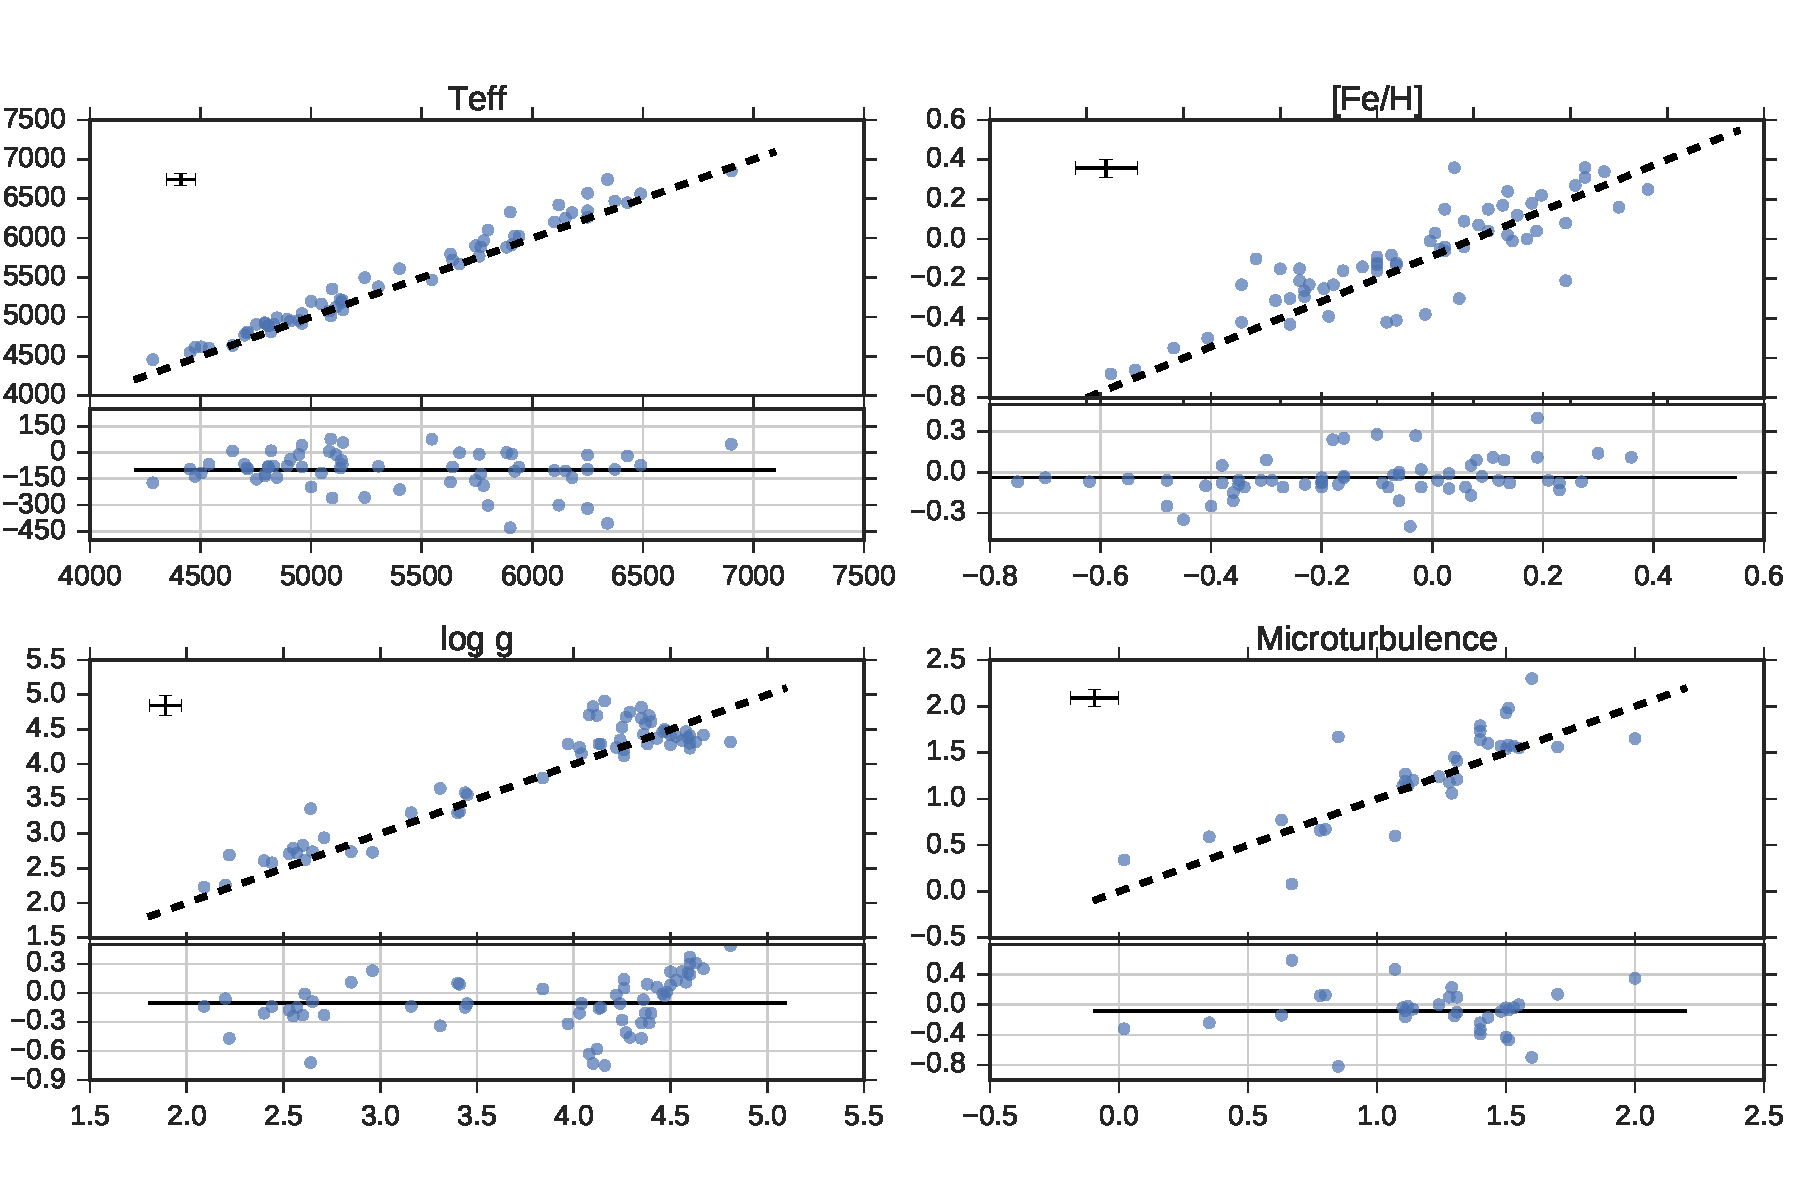
\includegraphics[width=1.0\linewidth,natwidth=870,natheight=580]{figures/update.pdf}
    \caption{Atmospheric parameters of the updated planet host stars. The x-axis
    are previous values, while the y-axis is the new updated values. In the
    upper left corner of each of the four plots we show the typical error
    on the parameters.}
    \label{fig:update}
\end{figure*}

The metallicity distribution for all the planet host stars are important to
understand e.g. planet formation. We present a distribution in
Figure~\ref{fig:distribution}. The sample is divided in two, for all stars, and
for stars brighter than 12 V magnitude. Stars dimmer are mainly observed with
the \emph{Kepler} space mission. These dim stars are very time consuming, and
hence expensive to observe.

\begin{figure}[tpb]
    \centering
    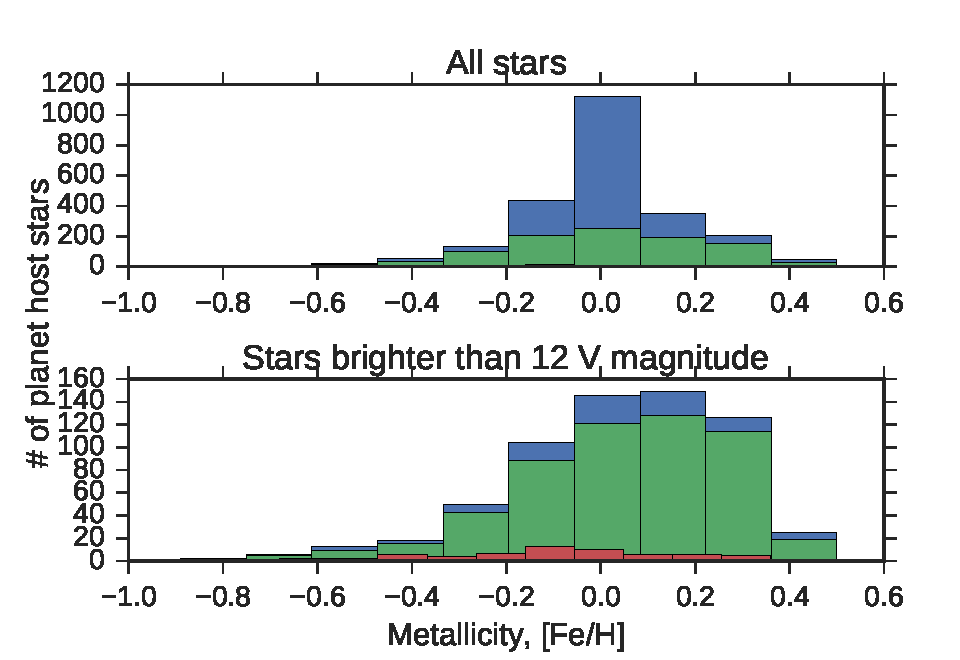
\includegraphics[width=1.0\linewidth,natwidth=450,natheight=300]{figures/metallicityDistribution.pdf}
    \caption{The metallicity distribution. In the \emph{upper} plot we see all
             stars (logarithmic scale) in SWEET-Cat, divided in three. Blue
             (the largest distribution) are all stars available in SWEET-Cat,
             green (the middle distribution) are the stars with homogenity flag
             1, i.e. analyzed using the method described in this paper, red
             (the smallest distribution) are all new stars added from this
             paper. The \emph{lower} plot show a 12 V magnitude cut to exclude
             stars which are currently unavailable spectroscopically.}
    \label{fig:distribution}
\end{figure}



\section{Discussion}
\label{sec:Discussion}
We will now focus on the stars with $T_\mathrm{eff}$ higher than \SI{4800}{K}
and lower than \SI{6500}{K}. Outside this range the EW method suffer from
different factors and will be less reliable. For the lower range, we expect to
see more line blending, and hence the EW measurements will no longer be
reliable. Without reliable EW measurements, the rest of the technique will not
work. For the other limit we start to see non-LTE effects which we do not take
into account, hence the method does not work there \citep{Gray2006}.

We compute radius and mass of all stars (even the ones which parameters may not
be reliable in order to be complete) using the empirical formula presented in
\citet{Torres2010}. Some of the stars have derived radius from different methods
and generally show a good correlation with radius derived from
\citet{Torres2010} if the literature parameters of $T_\mathrm{eff}$, $\log g$,
and $[\ion{Fe}/\ion{H}]$ are used. However, if we compare with the new radius
derived using the parameters presented here the results can differ up to 65\%.
We show in Figure~\ref{fig:RR} how the radius calculated from \citet{Torres2010}
differ between the literature atmospheric parameters and the new homogeneous
atmospheric parameters presented here. We note that stellar radii is provided by
many of the authors from different discovery papers, but we chose to compare the
atmospheric parameters via the derivation of the stellar radius as described
above, rather than compare the stellar radii from different methods.

\begin{figure}[tpb]
    \centering
    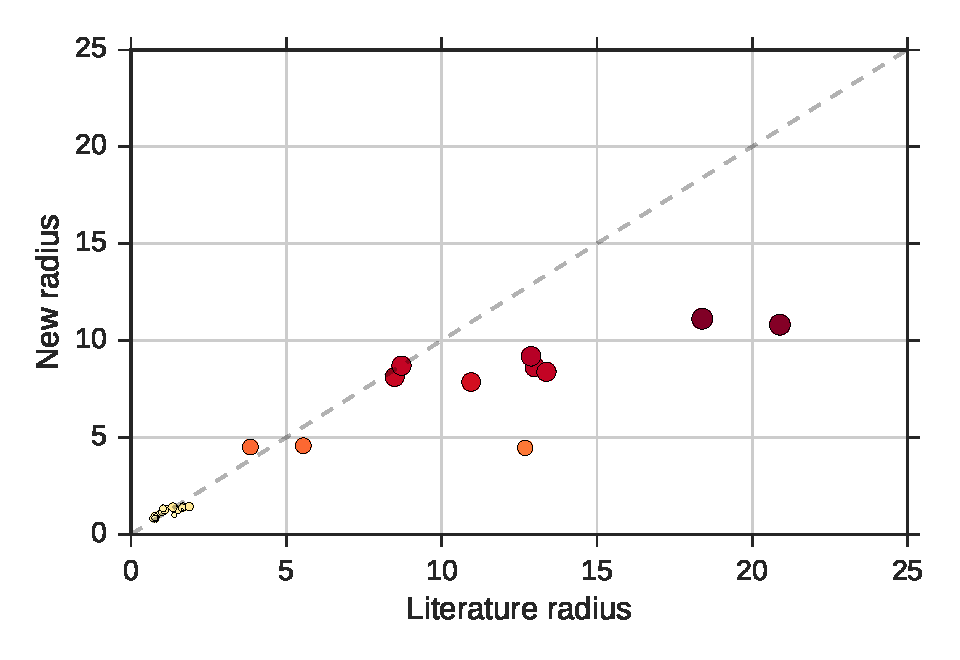
\includegraphics[width=1.0\linewidth]{figures/radiusVSradius.pdf}
    \caption{The stellar radius on both axis calculated based on \citet{Torres2010}.
    For the x-axis we show the stellar radius based on the atmoshperic parameters
    from the literature, while the y-axis is from the new homogeneous parameters
    presented here. The colour and size present the surface gravity. This clearly
    shows that the disagreement is biggest for more evolved stars.}
    \label{fig:RR}
\end{figure}

Below we discuss the systems where the radius of the stars change more then 25\%
and how this influence the planetary parameters. The changes in radius for a
star is primarily due to changes in $\log g$, which can be used as an indicator
of the evolutionary stage of a star.

The 7 stars (8 exoplanets) which radius deviates more than 25\% are discussed
below. We rederive the planetary radius, mass and semi-major axis when possible
following the three simple relations:

\begin{align}
    M_\mathrm{pl,new} &= \left(\frac{M_\mathrm{st,lit}}{M_\mathrm{st,new}}\right)^{-2/3} M_\mathrm{pl,lit}  \\
    R_\mathrm{pl,new} &= \left(\frac{R_\mathrm{st,lit}}{R_\mathrm{st,new}}\right) R_\mathrm{pl,lit} \\
    a_\mathrm{pl,new} &= \left(\frac{M_\mathrm{st,lit}}{M_\mathrm{st,new}}\right)^{1/3} a_\mathrm{pl,lit},
\end{align}
where subscript lit denotes the value from the literature which we compare with,
subscript new will be the new computed values, subscript pl is short for planet,
and last subscript st is short for star. $M$, $R$, and $a$ are mass, radius, and
semi-major axis respectively. Note that for the literature values, we use the
values reported directly from the literature, and not the derived radius and
mass from \citet{Torres2010}. To identify outliers, we compare radii and masses
derived from \citet{Torres2010} since this is a measure of how the atmospheric
parameters have changed.

\subsection{HAT-P-46}
\label{sub:HAT-P-46}
HAT-P-46 has two discovered exoplanets according to \citet{Hartmann2014}. The
outer planet HAT-P-46 c is not transiting hence we do not have any radius for
this planet. The results we present in this paper for this star comes from UVES
data with a SNR at 208. \citet{Hartmann2014} derives the following spectroscopic
parameters: $T_\mathrm{eff}=\SI{6120(100)}{K}$, $\log g=4.25\pm0.11$, and
$[\ion{Fe}/\ion{H}]=0.30\pm0.10$. We note that for this star the asteroseismic
correction we apply as mentioned in Section~\ref{sec:results}, the corrected
$\log g$ were below 4.2dex, so we end up using the spectroscopic $\log g$ for
this star.

If we derive the mass and radius of HAT-P-46 b with our new parameters, we
obtain the following: $R_\mathrm{pl} = 0.93$, while \citet{Hartmann2014} derived
$R_\mathrm{pl} = 1.28$ in units of Jupiter. We see no change in mass
(\citet{Hartmann2014} found $M_\mathrm{pl}=0.49$), however there is a decrease
in the radius, and we end up with a more dense planet, $\rho_\mathrm{pl}=0.76$
from $\rho_\mathrm{pl}=0.28\pm0.10$.

As the secondary companion does not transit we only have a limit on the minimum
mass for this planet. Here we get: $M\sin i_\mathrm{pl} = 1.97(2.00)$, so a very
small change as expected.


\subsection{HD 120084}
\label{sub:HD_120084}
The exoplanet orbiting this star with a period of 2082 days and quite eccentric
orbit at 0.66 was discovered by \citet{Sato2013}. Atmospheric parameters were
derived by \citet{Takeda2008} using a similar method as described in this paper.
The spectra they analyzed however, was not of as high quality as used here.
Using the HIDES spectrograph \citet{Takeda2008} reported an average SNR for
their sample of 100-300 at a resolving power of 67 000. We used data from
ESPaDOnS with a resolving power of 81 000, and with a SNR for this star of 850.
With our new parameter we obtain a slightly lower stellar mass for the star at
$1.93M_\odot$ compared to $2.39M_\odot$ obtained by \cite{Takeda2008}, hence the
minimum planetary mass is also decreased slightly from $m_\mathrm{pl}\sin
i=4.5m_J$ to $m_\mathrm{pl}\sin i=3.9m_J$. We see a decrease in the stellar
radius by 28\% from $9.12R_\odot$ to $7.81R_\odot$. Since there are no
observations of the planet transiting, the planetary radius has not been
computed.


\subsection{HD 233604}
\label{sub:HD_233604}
HD 233604 b was discovered by \citet{Nowak2013} while the atmospheric parameters
of the star were derived by \citet{Zielinski2012} with the same method as
described in this paper using the HRS spectrograph with a resolving power of 60
000 with a typical SNR at 200-250. We obtained the spectrum for this star using
the FIES spectrograph with a slightly higher resolution at 67 000, and similar
but also slightly higher SNR at 320 for this star.

This planet is very close orbit with a semi-major axis of $\sim 15R_\mathrm{st}$
($R_\mathrm{st}$ is the stellar radius) using the parameters from
\citet{Nowak2013}. With the updated parameters presented in this paper we see a
slight increase in the stellar mass from $1.5M_\odot$ to $1.9M_\odot$ and a
decrease in stellar radius from $10.5R_\odot$ to $8.6R_\odot$. This gives an
increase of the semi major axis to $\sim 21R_\mathrm{st}$. Note that the correct
stellar radius are used to describe the semi-major axis in both cases.

The increase in stellar mass leads to an increase in the minimum planetary mass,
from $6.58M_J$ to $7.79M_J$.

\citet{Nowak2013} found a high \ion{Li}{} abundance at
$A(\ion{Li}{})=1.400\pm0.042$ for this star speculating if this star might have
engulfed a planet. A more likely explanation is that this star has not yet
reached the first dredge-up process \citep{Nowak2013}. We found a much lower
value at $A(\ion{Li}{})=0.9$ and hence we find the star to not be \ion{Li}{}
rich. The \ion{Li}{} abundance we find is in excellent agreement with
\citet{Adamow2014} as we get the same abundance. They also calculate the
\ion{Li}{} abundance with a non-LTE correction and get $A(\ion{Li}{})=1.08$. To
understand this star in detail a more detailed abundance study would be needed
as well as a precise placement in an HR diagram.

\subsection{HD 5583}
\label{sub:HD_5583}
This exoplanet was discovered by \citet{Niedzielski2016} has an orbital period
of 139 days around a K giant. This exoplanet was discovered with the radial
velocity technique, hence we do not have a planetary radius. The stellar
parameters were derived in a similar manner as presented here
\citep[see][and references therein]{Niedzielski2016} where our biggest
disagreement is in the surface gravity. We derive a 0.34 dex higher $\log g$
giving us a smaller stellar radius (37\% smaller). The derived mass is 15\%
higher which in turn increases the minimum planetary mass from $5.78M_J$ to
$8.63M_J$. Even with the increase in mass, it is still within the planetary
regime for most inclinations as noted by \citet{Niedzielski2016}.



\subsection{HD 81688}
\label{sub:HD81688}
This exoplanet was discovered by \citet{Sato2008} with the RV method. The host
star is a metal-poor K giant. The atmospheric parameters presented in
\citet{Sato2008} are from the same method as presented in this paper, and we
have quite good agreement. Once again the big disagreement is in the surface
gravity where ours is 0.48 dex higher. Even though the stellar parameters, and
hence the planetary, does change, the radius and mass we derive are not far from
what is presented in the paper by \citet{Sato2008}. This is a case where the
star was marked as an outlier due to the comparison between the radius and mass
derived from \citet{Torres2010}.

The new stellar mass is the same as before, $2.1M\_dot$. The stellar radius
change from $13.0R_\odot$ to $10.8R_\odot$. Since a transit of this star has not
been observed and the stellar mass remains the same, we do not see any change in
the planetary parameters.

We note that this system is in an interesting configuration with a very close
orbit around an evolved star. This system, among others, have been subject
to work on planet engulfment \citep[see e.g.][]{Kunitomo2011}.


\subsection{HIP 107773}
\label{sub:HIP_107773}
The planetary companion were presented in \citet{Jones2015} as an exoplanet
around an intermediate mass evolved star. The stellar parameters were obtained
from the analysis by \citet{Jones2011} using the same method as presented here,
however with a different line list which might lead to some disagreements. For
this star we derive a higher $\log g$ at 2.83 dex compared to 2.60 dex, and thus
we derive a slightly smaller star with $11.6R_\odot$ to $9.2R_\odot$ and
$2.4M_\odot$ to $2.1M_\odot$ for radius and mass of the star respectively. The
other atmospheric parameters are very similar to those derived by
\citet{Jones2011}. This leads to a reduced minimum mass of the planetary
companion from $m\sin i=1.98M_J$ to $m\sin i=1.78M_J$.



\subsection{WASP-97}
\label{sub:WASP-97}
The exoplanet orbiting WASP-97 was discovered by \citet{Hellier2014}. The host
star parameters were derived in a similar method as described in this paper
after co-adding several spectra from the CORALIE spectrograph. They reach a
SNR of 100 with a spectral resolution of 50 000. The parameters presented here
comes from the UVES spectrograph with a SNR of more than 200.

The parameters does not change much for this planet. The planetary mass is
changed from $1.32M_J$ to $1.37M_J$ and the radius from $1.13R_J$ to $1.42R_J$.
This does affect the density quite a lot from $\SI{1.13}{g/cm^3}$ to
$\SI{0.59}{g/cm^3}$. This exoplanet is then in the same category as Saturn with
a density lower than water, however with a size slightly larger than Jupiter.


\subsection{$\omega$ Serpentis (ome Ser)}
\label{sub:ome_Ser}
The exoplanet orbiting this star with a period of 277 days and an eccentric
orbit at 0.11 was also presented by \citet{Sato2013}. The atmospheric parameters
were derived in the same way as for HD 120084. We used data from FIES with a
resolving power of 67 000, and with a SNR for this star of 1168. With our new
parameter we obtain a slightly higher stellar mass for the star at $2.19M_\odot$
compared to $2.17M_\odot$ obtained by \cite{Takeda2008}. This change is not
significant enough to change the minimum planetary mass at $m_\mathrm{pl}\sin
i=1.7m_J$. The stellar radius decrease with more than one solar radius, from
$12.3R_\odot$ to $11.1R_\odot$. However, since there are no observations of
exoplanet transiting, we can not see the change in the planetary radius.



\subsection{omi UMa}
\label{sub:omiUMa}
omi UMa b was discovered by \citet{Sato2012} using the RV method. The stellar
parameters are from \citet{Takeda2008} as discussed above. The spectrum used for
this star is from ESPaDOnS with a SNR of more than 500 compared to the 100-300
SNR reached for the large sample presented in \citet{Takeda2008}. The luminosity
and mass for omi UMa were obtained from theoreitcal evolutionary tracks
\citep[see][and references therein]{Sato2012}. The radius was then estimated
using the Stefan-Boltzmann relationship and the measured luminosity and
$T_\mathrm{eff}$.

The parameters presented here mainly differ in the surface gravity where ours is
0.72 dex higher at $\log g=3.36$. These leads to a big change in stellar mass
and radius from $3.1M_\odot$ to $1.6M_\odot$ and $14.1R_\odot$ to $4.5R_\odot$,
respectively. omi UMa b was reported to be the first planet candidate around a
star more massive than $3M_\odot$ by \citet{Sato2012}. With these updated
results, the minimum mass of the planet is now $m\sin i=2.7M_J$ whereas it was
$m\sin i=4.1M_J$ \citep{Sato2012}. The exoplanet is not reported to transit as
seen from Earth, so we do not have a radius for this exoplanet, which would have
changes a lot with these new results.



\section{Conclusion}
\label{sec:conclusion}

With this update we bring the completeness of SWEET-Cat for stars brighter than
magnitude 10 (V band) up to 85\% (77\% for stars brighter than 12). The
parameters are available for the public in an easy accessible form at
\url{https://www.astro.up.pt/resources/sweet-cat/} which is continuously
updated. The importance of the homogeneous analysis which we keep striving for
is shown in Figure~\ref{fig:RR} where we see quite different derived stellar
radius when the atmospheric parameters comes from different methods. As have
been discussed in Section~\ref{sec:Discussion} this has a direct impact on the
planetary parameters. It is of great importance to know the planetary parameters
very well, both for individual systems but also for an ensemble. With accurate
and precise planetary parameters we will be able to distinguish the different
possible composition, let it be gas giant, water worlds, or rocky planets.

Last we also provide an online tool to derive the stellar atmospheric parameters
using FASMA. We recommend to only use this tool for spectra and stars where this
method is working, i.e. high resolution spectra with a high SNR. The stars can
be FGK dwarfs and FGK subgiants/giants. We are working on applying this method
in the NIR in order to include M stars in the analysis for the numerous
up-comming spectrographs.



\begin{acknowledgements}

This work was supported by Funda\c{c}\~ao para a Ci\^encia e a Tecnologia (FCT)
through the research grants UID/FIS/04434/2013 and PTDC/FIS-AST/1526/2014.
N.C.S., and S.G.S. acknowledge the support from FCT through Investigador FCT
contracts of reference IF/00169/2012, and IF/00028/2014, respectively, and
POPH/FSE (EC) by FEDER funding through the program “Programa Operacional de
Factores de Competitividade - COMPETE”. E.D.M. and B.J.A. acknowledge the
support from FCT in form of the fellowship SFRH/BPD/76606/2011 and
SFRH/BPD/87776/2012, respectively. This work also benefit from the collaboration
of a cooperation project FCT/CAPES - 2014/2015 (FCT Proc 4.4.1.00 CAPES).

AM received funding from the European Union Seventh Framework Programme
(FP7/2007-2013) under grant agreement number 313014 (ETAEARTH).

This research has made use of the SIMBAD database operated at CDS, Strasbourg
(France).

\end{acknowledgements}


\bibpunct{(}{)}{;}{a}{}{,}
\bibliographystyle{aa}
\bibliography{thesis}

\appendix

\begin{longtab}
\begin{landscape}
\begin{longtable}{lllclclr}
    \caption{\label{tab:results} The derived parameters for the 66 stars in our
             sample. The SNR is measured by ARES.}\\
    \hline\hline
    Star  &  $T_\mathrm{eff}$ (K)  &  $\log g$ (dex)  &  $[\ion{Fe}/\ion{H}]$ (dex)  &  $\xi_\mathrm{micro}$ (km/s)  &  $\xi_\mathrm{micro}$ fixed?  &  Instrument  &  SNR \\
    \hline
    \endfirsthead
    \caption{continued.}\\
    \hline
    \endhead
    \hline
    \endfoot
    \object{11 Com}         &   $4903 \pm 34 $   &  $2.55 \pm 0.13$\tablefootmark{a} &  $-0.23 \pm 0.03$  &  $1.56 \pm 0.04$  & no   &  FIES             &  966  \\
\object{14 And}         &   $4808 \pm 39 $   &  $2.61 \pm 0.10$\tablefootmark{a} &  $-0.22 \pm 0.03$  &  $1.60 \pm 0.04$  & no   &  FIES             &  724  \\
\object{42 Dra}         &   $4528 \pm 57 $   &  $2.27 \pm 0.11$\tablefootmark{a} &  $-0.30 \pm 0.03$  &  $1.53 \pm 0.05$  & no   &  FIES             &  645  \\
\object{BD -11 4672}    &   $4553 \pm 75 $   &  $4.87 \pm 0.51$                  &  $-0.30 \pm 0.02$  &  $0.14 \pm 0.07$  & yes  &  FIES             &  487  \\
\object{BD +49  828}    &   $5015 \pm 36 $   &  $2.87 \pm 0.09$\tablefootmark{a} &  $-0.01 \pm 0.03$  &  $1.48 \pm 0.04$  & no   &  FIES             &  567  \\
\object{GJ 785}         &   $5087 \pm 48 $   &  $4.42 \pm 0.10$                  &  $-0.01 \pm 0.03$  &  $0.69 \pm 0.10$  & no   &  HARPS            &  801  \\
\object{HATS-1}         &   $5969 \pm 46 $   &  $4.39 \pm 0.06$                  &  $-0.04 \pm 0.04$  &  $1.06 \pm 0.08$  & no   &  UVES             &  155  \\
\object{HATS-5}         &   $5383 \pm 91 $   &  $4.41 \pm 0.22$                  &  $ 0.08 \pm 0.06$  &  $0.91 \pm 0.14$  & no   &  UVES             &  158  \\
\object{HAT-P-12}       &   $4642 \pm 106$   &  $4.53 \pm 0.27$                  &  $-0.26 \pm 0.06$  &  $0.28 \pm 0.63$  & no   &  FIES             &  185  \\
\object{HAT-P-24}       &   $6470 \pm 181$   &  $4.33 \pm 0.27$                  &  $-0.41 \pm 0.10$  &  $1.40 \pm 0.03$  & yes  &  UVES             &  158  \\[5pt]
\object{HAT-P-39}       &   $6745 \pm 236$   &  $4.39 \pm 0.47$                  &  $-0.21 \pm 0.12$  &  $1.53 \pm 0.04$  & yes  &  UVES             &  127  \\
\object{HAT-P-42}       &   $5903 \pm 66 $   &  $4.29 \pm 0.10$\tablefootmark{a} &  $ 0.34 \pm 0.05$  &  $1.19 \pm 0.08$  & no   &  UVES             &  130  \\
\object{HAT-P-46}       &   $6421 \pm 121$   &  $4.53 \pm 0.14$\tablefootmark{a} &  $ 0.16 \pm 0.09$  &  $1.67 \pm 0.18$  & no   &  UVES             &  208  \\
\object{HD 102272}      &   $4883 \pm 34 $   &  $2.69 \pm 0.07$\tablefootmark{a} &  $-0.29 \pm 0.03$  &  $1.54 \pm 0.04$  & no   &  FIES             & 1011  \\
\object{HD 104985}      &   $4786 \pm 58 $   &  $2.66 \pm 0.09$\tablefootmark{a} &  $-0.28 \pm 0.04$  &  $1.65 \pm 0.05$  & no   &  FIES             & 1010  \\
\object{HD 114762}      &   $5879 \pm 39 $   &  $4.23 \pm 0.04$\tablefootmark{a} &  $-0.66 \pm 0.03$  &  $1.16 \pm 0.07$  & no   &  FIES             & 1671  \\
\object{HD 120084}      &   $4969 \pm 40 $   &  $2.94 \pm 0.14$\tablefootmark{a} &  $ 0.12 \pm 0.03$  &  $1.41 \pm 0.04$  & no   &  ESPaDOnS         &  852  \\
\object{HD 152581}      &   $5181 \pm 27 $   &  $3.37 \pm 0.06$\tablefootmark{a} &  $-0.23 \pm 0.02$  &  $1.15 \pm 0.03$  & no   &  FIES             &  796  \\
\object{HD 155358}      &   $5906 \pm 33 $   &  $4.24 \pm 0.03$\tablefootmark{a} &  $-0.61 \pm 0.02$  &  $1.30 \pm 0.05$  & no   &  FIES             &  424  \\
\object{HD 171028}      &   $5699 \pm 36 $   &  $3.83 \pm 0.03$\tablefootmark{a} &  $-0.40 \pm 0.02$  &  $1.21 \pm 0.04$  & no   &  FIES             &  460  \\[5pt]
\object{HD 192263}      &   $4946 \pm 46 $   &  $4.61 \pm 0.14$                  &  $-0.05 \pm 0.02$  &  $0.66 \pm 0.12$  & no   &  HARPS            &  415  \\
\object{HD 192699}      &   $5208 \pm 27 $   &  $3.56 \pm 0.10$\tablefootmark{a} &  $-0.12 \pm 0.02$  &  $1.19 \pm 0.03$  & no   &  FIES             &  776  \\
\object{HD 197037}      &   $6233 \pm 45 $   &  $4.22 \pm 0.04$                  &  $-0.12 \pm 0.03$  &  $1.22 \pm 0.06$  & no   &  FIES             & 1074  \\
\object{HD 200964}      &   $5083 \pm 24 $   &  $3.32 \pm 0.07$\tablefootmark{a} &  $-0.16 \pm 0.02$  &  $1.18 \pm 0.03$  & no   &  FIES             & 1081  \\
\object{HD 219134}      &   $4767 \pm 70 $   &  $4.57 \pm 0.17$                  &  $ 0.00 \pm 0.04$  &  $0.59 \pm 0.24$  & no   &  ESPaDOnS         &  725  \\
\object{HD 220074}      &   $4748 \pm 233$   &  $3.67 \pm 0.33$\tablefootmark{a} &  $-0.06 \pm 0.09$  &  $2.82 \pm 0.37$  & no   &  FIES             &  419  \\
\object{HD 220842}      &   $5999 \pm 39 $   &  $4.30 \pm 0.06$\tablefootmark{a} &  $-0.08 \pm 0.03$  &  $1.21 \pm 0.05$  & no   &  FIES             &  459  \\
\object{HD 233604}      &   $4954 \pm 46 $   &  $2.86 \pm 0.11$\tablefootmark{a} &  $-0.14 \pm 0.04$  &  $1.61 \pm 0.05$  & no   &  FIES             &  314  \\
\object{HD 283668}      &   $4841 \pm 73 $   &  $4.51 \pm 0.18$                  &  $-0.74 \pm 0.04$  &  $0.16 \pm 0.61$  & no   &  FIES             &  592  \\
\object{HD 285507}      &   $4620 \pm 126$   &  $4.72 \pm 0.61$                  &  $ 0.04 \pm 0.06$  &  $0.74 \pm 0.43$  & no   &  UVES             &  239  \\[5pt]
\object{HD 37124}       &   $5460 \pm 35 $   &  $4.24 \pm 0.04$                  &  $-0.42 \pm 0.03$  &  $0.61 \pm 0.07$  & no   &  FIES             &  988  \\
\object{HD 5583}        &   $4986 \pm 35 $   &  $2.87 \pm 0.09$\tablefootmark{a} &  $-0.35 \pm 0.03$  &  $1.62 \pm 0.04$  & no   &  FIES             &  933  \\
\object{HD 70573}       &   $5889 \pm 186$   &  $4.32 \pm 0.27$\tablefootmark{a} &  $-0.42 \pm 0.13$  &  $1.14 \pm 0.01$  & yes  &  FIES             &  487  \\
\object{HD 81688}       &   $4903 \pm 21 $   &  $2.70 \pm 0.05$\tablefootmark{a} &  $-0.21 \pm 0.02$  &  $1.54 \pm 0.02$  & no   & \tablefootmark{b} & 1350, 860  \\
\object{HD 82886}       &   $5123 \pm 18 $   &  $3.30 \pm 0.04$\tablefootmark{a} &  $-0.25 \pm 0.01$  &  $1.16 \pm 0.02$  & no   & \tablefootmark{c} & 1198,1294  \\
\object{HD 96063}       &   $5232 \pm 36 $   &  $3.61 \pm 0.06$\tablefootmark{a} &  $-0.12 \pm 0.03$  &  $1.23 \pm 0.04$  & no   &  FIES             &  644  \\
\object{HD 97658}       &   $5219 \pm 54 $   &  $4.60 \pm 0.10$                  &  $-0.28 \pm 0.04$  &  $0.78 \pm 0.11$  & no   &  FIES             & 1123  \\
\object{HD 87883}       &   $4917 \pm 68 $   &  $4.53 \pm 0.19$                  &  $ 0.02 \pm 0.03$  &  $0.46 \pm 0.21$  & no   &  ESPaDOnS         &  753  \\
\object{HIP 107773}     &   $4957 \pm 49 $   &  $2.83 \pm 0.09$\tablefootmark{a} &  $ 0.04 \pm 0.04$  &  $1.49 \pm 0.05$  & no   &  UVES             &  218  \\
\object{HIP 11915}      &   $5770 \pm 14 $   &  $4.33 \pm 0.03$                  &  $-0.06 \pm 0.01$  &  $0.95 \pm 0.02$  & no   &  HARPS            &  709  \\[5pt]
\object{HIP 116454}     &   $5038 \pm 82 $   &  $4.53 \pm 0.18$                  &  $-0.12 \pm 0.04$  &  $0.74 \pm 0.15$  & no   &  FIES             &  309  \\
\object{HR 228}         &   $5042 \pm 42 $   &  $3.30 \pm 0.09$\tablefootmark{a} &  $ 0.07 \pm 0.03$  &  $1.14 \pm 0.04$  & no   &  UVES             &  400  \\
\object{KELT-6}         &   $6246 \pm 88 $   &  $4.22 \pm 0.09$\tablefootmark{a} &  $-0.22 \pm 0.06$  &  $1.66 \pm 0.13$  & no   &  FIES             &  374  \\
\object{Kepler-37}      &   $5378 \pm 53 $   &  $4.47 \pm 0.12$                  &  $-0.23 \pm 0.04$  &  $0.58 \pm 0.13$  & no   &  FIES             &  205  \\
\object{Kepler-444}     &   $5111 \pm 43 $   &  $4.50 \pm 0.13$                  &  $-0.51 \pm 0.03$  &  $0.37 \pm 0.15$  & no   &  FIES             &  675  \\
\object{ksi Aql}        &   $4834 \pm 42 $   &  $2.65 \pm 0.10$\tablefootmark{a} &  $-0.14 \pm 0.03$  &  $1.53 \pm 0.04$  & no   &  FIES             &  919  \\
\object{mu Leo}         &   $4605 \pm 94 $   &  $2.61 \pm 0.26$\tablefootmark{a} &  $ 0.25 \pm 0.06$  &  $1.64 \pm 0.11$  & no   &  ESPaDOnS         &  354  \\
\object{ome Ser}        &   $4928 \pm 35 $   &  $2.69 \pm 0.06$\tablefootmark{a} &  $-0.11 \pm 0.03$  &  $1.55 \pm 0.04$  & no   &  FIES             & 1168  \\
\object{omi CrB}        &   $4882 \pm 40 $   &  $2.64 \pm 0.10$\tablefootmark{a} &  $-0.17 \pm 0.03$  &  $1.55 \pm 0.04$  & no   &  FIES             &  932  \\
\object{omi UMa}        &   $5499 \pm 52 $   &  $3.36 \pm 0.07$\tablefootmark{a} &  $-0.01 \pm 0.05$  &  $1.98 \pm 0.06$  & no   &  ESPaDOnS         &  527  \\[5pt]
\object{Qatar-}2        &   $4637 \pm 316$   &  $4.53 \pm 0.62$                  &  $ 0.09 \pm 0.17$  &  $0.63 \pm 0.83$  & no   &  UVES             &   97  \\
\object{SAND364}        &   $4457 \pm 104$   &  $2.26 \pm 0.20$\tablefootmark{a} &  $-0.04 \pm 0.06$  &  $1.60 \pm 0.11$  & no   &  UVES             &  220  \\
\object{TYC+1422-614-1} &   $4908 \pm 41 $   &  $2.90 \pm 0.12$\tablefootmark{a} &  $-0.07 \pm 0.03$  &  $1.57 \pm 0.05$  & no   &  FIES             &  506  \\
\object{WASP-37}        &   $5917 \pm 72 $   &  $4.25 \pm 0.15$                  &  $-0.23 \pm 0.05$  &  $0.59 \pm 0.13$  & no   &  FIES             &  232  \\
\object{WASP-44}        &   $5612 \pm 80 $   &  $4.39 \pm 0.30$                  &  $ 0.17 \pm 0.06$  &  $1.32 \pm 0.13$  & no   &  UVES             &  125  \\
\object{WASP-52}        &   $5197 \pm 83 $   &  $4.55 \pm 0.30$                  &  $ 0.15 \pm 0.05$  &  $1.16 \pm 0.14$  & no   &  UVES             &  125  \\
\object{WASP-58}        &   $6039 \pm 55 $   &  $4.23 \pm 0.10$                  &  $-0.09 \pm 0.04$  &  $1.12 \pm 0.08$  & no   &  FIES             &  310  \\
\object{WASP-61}        &   $6265 \pm 168$   &  $4.21 \pm 0.21$\tablefootmark{a} &  $-0.38 \pm 0.11$  &  $1.44 \pm 0.02$  & yes  &  UVES             &  163  \\
\object{WASP-72}        &   $6570 \pm 85 $   &  $4.25 \pm 0.13$                  &  $ 0.15 \pm 0.06$  &  $2.30 \pm 0.15$  & no   &  UVES             &  174  \\
\object{WASP-75}        &   $6203 \pm 46 $   &  $4.42 \pm 0.22$\tablefootmark{a} &  $ 0.24 \pm 0.03$  &  $1.45 \pm 0.06$  & no   &  UVES             &  189  \\[5pt]
\object{WASP-76}        &   $6347 \pm 52 $   &  $4.29 \pm 0.08$\tablefootmark{a} &  $ 0.36 \pm 0.04$  &  $1.73 \pm 0.06$  & no   &  UVES             &  165  \\
\object{WASP-82}        &   $6563 \pm 55 $   &  $4.29 \pm 0.10$\tablefootmark{a} &  $ 0.18 \pm 0.04$  &  $1.93 \pm 0.08$  & no   &  UVES             &  239  \\
\object{WASP-88}        &   $6450 \pm 61 $   &  $4.24 \pm 0.06$\tablefootmark{a} &  $ 0.03 \pm 0.04$  &  $1.79 \pm 0.09$  & no   &  UVES             &  174  \\
\object{WASP-95}        &   $5799 \pm 31 $   &  $4.29 \pm 0.05$\tablefootmark{a} &  $ 0.22 \pm 0.03$  &  $1.18 \pm 0.04$  & no   &  UVES             &  247  \\
\object{WASP-97}        &   $5723 \pm 52 $   &  $4.24 \pm 0.07$                  &  $ 0.31 \pm 0.04$  &  $1.03 \pm 0.08$  & no   &  UVES             &  219  \\
\object{WASP-99}        &   $6324 \pm 89 $   &  $4.34 \pm 0.12$                  &  $ 0.27 \pm 0.06$  &  $1.83 \pm 0.12$  & no   &  UVES             &  249  \\

\end{longtable}
\tablefoot{
\tablefoottext{a}{Spectroscopic $\log g$.}
\tablefoottext{b}{Weighted average of ESPaDoNS and FIES results. The parameters
                  are (FIES in parantheses):
                  $T_\mathrm{eff}=4870(4934)\pm30(29)$,
                  $\log g=2.50(2.73)\pm0.14(0.05)$,
                  $[\ion{Fe}/\ion{H}]=-0.26(-0.19)\pm0.03(0.02)$, and
                  $\xi_\mathrm{micro}=1.50(1.59)\pm0.03(0.03)$.}
\tablefoottext{c}{Weighted average of ESPaDoNS and FIES results. The parameters
                  are (FIES in parantheses):
                  $T_\mathrm{eff}=15124(5121)\pm22(29)$,
                  $\log g=3.30(3.31)\pm0.05(0.07)$,
}}
\end{landscape}
\end{longtab}


\end{document}
